% !TeX program = xelatex
\documentclass[a4paper,10pt]{article}

% ============================================================================
% កញ្ចប់បណ្ណាល័យ (Packages) – តាមលំនាំស្តង់ដារ អនុវិទ្យាល័យព្រះក្រសាំង (ls_plan.tex)
% បរិបទ៖ ថ្នាក់រៀនគ្មានស្លាយ LCD – បង្រៀនដោយប្រើក្ដារខៀន ដែកឈាន និងសន្លឹកកិច្ចការសិស្សស-ខ្មៅជាគោល
% ============================================================================
\usepackage[a4paper, left=0.95cm, right=0.95cm, top=0.85cm, bottom=0.92cm, footskip=0.52cm]{geometry}
\usepackage{amsmath}
\usepackage{unicode-math}
\usepackage{fontspec}
\usepackage{array, longtable, multirow, colortbl}
\usepackage[table]{xcolor}
\usepackage{enumitem}
\usepackage{pifont}
\usepackage{fancyhdr}
\usepackage{tikz}
\usetikzlibrary{calc, arrows.meta, angles, quotes, decorations.markings, positioning, babel}

\makeatletter
\let\@expl@@@mark@update@singlecol@structures@@\relax
\makeatother

% ============================================================================
% ការកំណត់ពុម្ពអក្សរផ្លូវការ (Cross-Platform Fonts Configuration)
% ============================================================================
\providecommand{\NGSFindFonts}{%
  \IfFileExists{C:/Windows/Fonts/cambria.ttc}{%
    \def\NGSSysPath{C:/Windows/Fonts/}%
    \def\NGSUserPath{C:/Users/KIT/AppData/Local/Microsoft/Windows/Fonts/}%
  }{%
    \IfFileExists{./fonts/KhmerOSsiemreap.ttf}{\def\NGSSysPath{./fonts/}\def\NGSUserPath{./fonts/}}{%
    \IfFileExists{../fonts/KhmerOSsiemreap.ttf}{\def\NGSSysPath{../fonts/}\def\NGSUserPath{../fonts/}}{%
    \IfFileExists{../../fonts/KhmerOSsiemreap.ttf}{\def\NGSSysPath{../../fonts/}\def\NGSUserPath{../../fonts/}}{%
    \IfFileExists{../../../fonts/KhmerOSsiemreap.ttf}{\def\NGSSysPath{../../../fonts/}\def\NGSUserPath{../../../fonts/}}{%
    \IfFileExists{../../../../fonts/KhmerOSsiemreap.ttf}{\def\NGSSysPath{../../../../fonts/}\def\NGSUserPath{../../../../fonts/}}{%
    \IfFileExists{../../../../../fonts/KhmerOSsiemreap.ttf}{\def\NGSSysPath{../../../../../fonts/}\def\NGSUserPath{../../../../../fonts/}}{%
    \IfFileExists{../../../../../../fonts/KhmerOSsiemreap.ttf}{\def\NGSSysPath{../../../../../../fonts/}\def\NGSUserPath{../../../../../../fonts/}}{%
      \def\NGSSysPath{../../../../../../../fonts/}\def\NGSUserPath{../../../../../../../fonts/}%
    }}}}}}}%
  }%
}
\NGSFindFonts

\setmathfont[Path={\NGSSysPath}, FontIndex=1, Scale=1.02]{cambria.ttc}
\defaultfontfeatures{Ligatures=TeX}

\setmainfont[
  Path={\NGSUserPath},
  Extension=.ttf,
  Script=Khmer,
  BoldFont={KhmerOSsiemreap},
  BoldFeatures={FakeBold=1.8},
  ItalicFont={KhmerOSsiemreap},
  ItalicFeatures={FakeSlant=0.25},
  BoldItalicFont={KhmerOSsiemreap},
  BoldItalicFeatures={FakeBold=1.8, FakeSlant=0.25}
]{KhmerOSsiemreap}

\newfontfamily\muol[Path={\NGSUserPath}, Extension=.ttf, Script=Khmer]{KhmerOSmuollight}
\newfontfamily\TimesEn[Path={\NGSSysPath}, Extension=.ttf, BoldFont={timesbd}, ItalicFont={timesi}, BoldItalicFont={timesbi}]{times}
\newfontfamily\NagaBold[Path={\NGSUserPath}, Extension=.ttf]{AKbalthom Naga Bold}
\newfontfamily\CalibriFont[Path={\NGSSysPath}, Extension=.ttf]{calibri}
\newfontfamily\Tacteing[Path={\NGSUserPath}]{TACTENG.TTF}
\newfontfamily\CourierBullet[Path={\NGSSysPath}, Extension=.ttf]{cour}
\newcommand{\wcirc}{{\CourierBullet\fontsize{9.5pt}{11pt}\selectfont o}}

\XeTeXlinebreaklocale "km"
\XeTeXlinebreakskip = 0pt plus 1pt minus 0.1pt

\definecolor{stepgray}{HTML}{D9D9D9}
\definecolor{headgray}{HTML}{F2F2F2}
\definecolor{boxgray}{HTML}{D9D9D9}
\definecolor{darkred}{HTML}{C00000}
\definecolor{red5e}{HTML}{FF0000}

\pagestyle{fancy}
\fancyhf{}
\renewcommand{\headrulewidth}{0pt}
\fancyfoot[R]{\CalibriFont\fontsize{11pt}{13pt}\selectfont\thepage}

\setlength{\parindent}{0pt}
\setlength{\parskip}{0pt}
\setlength{\tabcolsep}{3.8pt}

\newcolumntype{L}[1]{>{\raggedright\arraybackslash}p{#1}}

\newcommand{\en}[1]{{\TimesEn #1}}
\newcommand{\enbf}[1]{{\TimesEn\textbf{#1}}}
\newcommand{\unit}[1]{\,\text{\en{#1}}}
\newcommand{\fiveE}[1]{{\NagaBold\fontsize{9.5pt}{13pt}\selectfont\textcolor{red5e}{#1}}}
\newcommand{\timenote}[1]{\textcolor{darkred}{\textit{#1}}}
\newcommand{\graybox}[1]{\colorbox{boxgray}{\strut\hspace{2pt}#1\hspace{2pt}}}
\newcommand{\ditem}{\tikz[baseline=-0.5ex]\fill (0,0.42ex) -- (0.42ex,0) -- (0,-0.42ex) -- (-0.42ex,0) -- cycle;\hspace{0.3em}}
\newcommand{\cnum}[1]{{\fontsize{10.5pt}{12pt}\selectfont\ding{\numexpr171+#1\relax}}\hspace{0.2em}}
\newcommand{\cfig}[1]{\par\vspace{4pt}{\centering #1\par}\vspace{4pt}}
\newcommand{\stepheader}[1]{\multicolumn{3}{|c|}{\cellcolor{stepgray}\muol #1} \\* \noalign{\hrule height 0.4pt}}
\newcommand{\tri}[1]{\ensuremath{\triangle #1}}
\newcommand{\ang}[1]{\ensuremath{\angle #1}}
\newcommand{\arc}[1]{\ensuremath{\widehat{#1}}}
\newcommand{\cg}{\ensuremath{\cong}}
\newcommand{\khmflourish}{{\Tacteing\fontsize{36pt}{14pt}\selectfont\raisebox{-5pt}{3}}}

\tikzset{
  tk1/.style={postaction={decorate},decoration={markings,mark=at position 0.50 with {\draw[black, line width=0.85pt](0,-0.095)--(0,0.095);}}},
  tk2/.style={postaction={decorate},decoration={markings,
    mark=at position 0.45 with {\draw[black, line width=0.85pt](0,-0.095)--(0,0.095);},
    mark=at position 0.55 with {\draw[black, line width=0.85pt](0,-0.095)--(0,0.095);}}}
}

% ============================================================================
% ម៉ាក្រូរូបភាពធរណីមាត្រស-ខ្មៅ (Proportional 4.2–7.2 cm B&W TikZ Diagrams)
% ============================================================================

% ១. E1 Engage + រំលឹកមេដ្យាទ័រ៖ បំណែកចានបុរាណបាក់មានចំណុចគែម A, B, C
\newcommand{\figEngageCIRCOne}{%
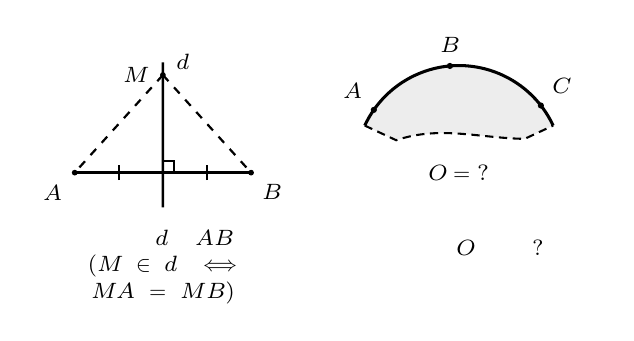
\begin{tikzpicture}[scale=0.80, every node/.style={font=\footnotesize, text=black}]
  % ឆ្វេង៖ រំលឹកមេដ្យាទ័រនៃអង្កត់ AB (មេរៀនទី១២)
  \begin{scope}[shift={(0,0)}]
    \coordinate (A) at (0,0.6); \coordinate (B) at (2.8,0.6);
    \coordinate (I) at (1.4,0.6); \coordinate (M) at (1.4,2.15);
    \draw[black, line width=0.95pt, tk1] (A)--(I);
    \draw[black, line width=0.95pt, tk1] (I)--(B);
    \draw[black, line width=0.95pt] (I) ++(0,-0.55) -- (1.4,2.35) node[right=1pt] {$d$};
    \draw[black, line width=0.8pt, dashed] (M)--(A) (M)--(B);
    \draw[black, line width=0.7pt] (1.4,0.6) rectangle ++(0.18,0.18);
    \fill[black] (A) circle (1.3pt) node[below left=1pt] {$A$};
    \fill[black] (B) circle (1.3pt) node[below right=1pt] {$B$};
    \fill[black] (M) circle (1.3pt) node[left=2pt] {$M$};
    \node[anchor=north, text width=3.2cm, align=center] at (1.4,-0.15) {មេដ្យាទ័រ $d$ នៃ $AB$\\($M\in d \iff MA=MB$)};
  \end{scope}
  % ស្ដាំ៖ បេសកកម្ម E1 បំណែកចានបុរាណកាត់តាម A, B, C
  \begin{scope}[shift={(4.45,0)}]
    \coordinate (O) at (1.65,0.65);
    \fill[gray!14] (O) ++(25:1.65) arc (25:155:1.65) -- ($(O)+(155:1.10)$) .. controls (1.35,1.35) and (1.95,1.15) .. ($(O)+(25:1.15)$) -- cycle;
    \draw[black, line width=1.1pt] (O) ++(25:1.65) arc (25:155:1.65);
    \draw[black, line width=0.75pt, densely dashed] ($(O)+(155:1.65)$) -- ($(O)+(155:1.10)$) .. controls (1.35,1.35) and (1.95,1.15) .. ($(O)+(25:1.15)$) -- ($(O)+(25:1.65)$);
    \coordinate (C1) at ($(O)+(38:1.65)$);
    \coordinate (B1) at ($(O)+(95:1.65)$);
    \coordinate (A1) at ($(O)+(145:1.65)$);
    \fill[black] (A1) circle (1.4pt) node[above left=1pt] {$A$};
    \fill[black] (B1) circle (1.4pt) node[above=1.5pt] {$B$};
    \fill[black] (C1) circle (1.4pt) node[above right=1pt] {$C$};
    \node at (1.65,0.60) {$O=?$};
    \node[anchor=north, text width=3.5cm, align=center] at (1.65,-0.15) {បំណែកគែមចានបុរាណ\\តើរកផ្ចិតដើម $O$ ដូចម្ដេច?};
  \end{scope}
\end{tikzpicture}}

% ១ប. E2 Explore: ឧទាហរណ៍ទី២ ទំ.១៩៨ (កាត់តាម ២ ចំណុច A, B) + អន្ទាក់ ៣ ចំណុចរត់ត្រង់គ្នា (d1 || d2)
\newcommand{\figExploreLocusCIRCOne}{%
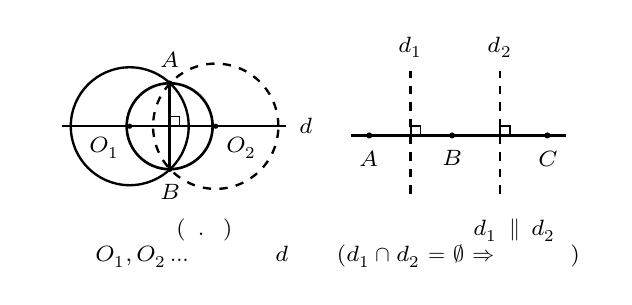
\begin{tikzpicture}[scale=0.78, every node/.style={font=\footnotesize, text=black}]
  % ឆ្វេង៖ រង្វង់ច្រើនកាត់តាម A និង B (ផ្ចិតលើមេដ្យាទ័រ ទំ.១៩៨)
  \begin{scope}[shift={(0,0)}]
    \coordinate (A) at (1.50,1.95); \coordinate (B) at (1.50,0.55);
    \coordinate (M) at (1.50,1.25);
    \coordinate (O1) at (0.85,1.25); \coordinate (O2) at (1.50,1.25); \coordinate (O3) at (2.25,1.25);
    \draw[black, line width=0.85pt] (O1) circle (0.96);
    \draw[black, line width=0.95pt] (O2) circle (0.70);
    \draw[black, line width=0.85pt, dashed] (O3) circle (1.02);
    \draw[black, line width=0.90pt] (A)--(B);
    \draw[black, line width=0.85pt] (-0.25,1.25)--(3.40,1.25) node[right=1pt] {$d$};
    \draw[black, line width=0.65pt] (1.50,1.25) rectangle ++(0.16,0.16);
    \fill[black] (A) circle (1.3pt) node[above=2pt] {$A$};
    \fill[black] (B) circle (1.3pt) node[below=2pt] {$B$};
    \fill[black] (O1) circle (1.2pt) node[below left=0.5pt] {$O_1$};
    \fill[black] (O3) circle (1.2pt) node[below right=0.5pt] {$O_2$};
    \node[anchor=north, text width=3.45cm, align=center] at (1.55,-0.10) {ឧទាហរណ៍ទី២ (ទំ.១៩៨)៖\\ផ្ចិត $O_1, O_2\dots$ លើមេដ្យាទ័រ $d$};
  \end{scope}
  % ស្ដាំ៖ អន្ទាក់ ៣ ចំណុចរត់ត្រង់គ្នា => d1 || d2 គ្មានផ្ចិតប្រសព្វ
  \begin{scope}[shift={(4.55,0)}]
    \coordinate (A) at (0.20,1.10); \coordinate (B) at (1.55,1.10); \coordinate (C) at (3.10,1.10);
    \coordinate (I1) at (0.875,1.10); \coordinate (I2) at (2.325,1.10);
    \draw[black, line width=1.0pt] (-0.10,1.10)--(3.40,1.10);
    \draw[black, line width=0.90pt, dashed] (0.875,0.15)--(0.875,2.15) node[above=1pt] {$d_1$};
    \draw[black, line width=0.90pt, dashed] (2.325,0.15)--(2.325,2.15) node[above=1pt] {$d_2$};
    \draw[black, line width=0.65pt] (I1) rectangle ++(0.16,0.16);
    \draw[black, line width=0.65pt] (I2) rectangle ++(0.16,0.16);
    \fill[black] (A) circle (1.4pt) node[below=2pt] {$A$};
    \fill[black] (B) circle (1.4pt) node[below=2pt] {$B$};
    \fill[black] (C) circle (1.4pt) node[below=2pt] {$C$};
    \node[anchor=north, text width=3.45cm, align=center] at (1.65,-0.10) {ករណីរត់ត្រង់គ្នា៖ $d_1 \parallel d_2$\\($d_1\cap d_2=\varnothing \Rightarrow$ គ្មានរង្វង់)};
  \end{scope}
\end{tikzpicture}}

% ២. E3 Explain: ធាតុនៃរង្វង់ C(O,r) (ទំ.១៩៧) និងការកំណត់រង្វង់តាម ៣ ចំណុច (ទំ.១៩៨)
\newcommand{\figCircleDefDet}{%
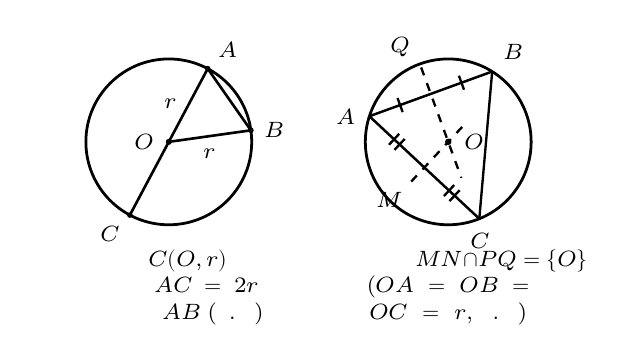
\begin{tikzpicture}[scale=0.78, every node/.style={font=\footnotesize, text=black}]
  % ឆ្វេង៖ និយមន័យ C(O,r) កាំ អង្កត់ធ្នូ អង្កត់ផ្ចិត (ទំ.១៩៧)
  \begin{scope}[shift={(0,0)}]
    \coordinate (O) at (1.55,1.45);
    \draw[black, line width=1.0pt] (O) circle (1.35);
    \coordinate (A) at ($(O)+(62:1.35)$);
    \coordinate (C) at ($(O)+(242:1.35)$);
    \coordinate (B) at ($(O)+(8:1.35)$);
    \draw[black, line width=0.95pt] (A)--(C);
    \draw[black, line width=0.95pt] (A)--(B) (O)--(B);
    \fill[black] (O) circle (1.4pt) node[left=2pt] {$O$};
    \fill[black] (A) circle (1.3pt) node[above right=0.5pt] {$A$};
    \fill[black] (B) circle (1.3pt) node[right=1.5pt] {$B$};
    \fill[black] (C) circle (1.3pt) node[below left=0.5pt] {$C$};
    \node[left=1pt] at ($(O)!0.52!(A)$) {$r$};
    \node[below=1pt] at ($(O)!0.50!(B)$) {$r$};
    \node[anchor=north, text width=3.35cm, align=center] at (1.55,-0.15) {រង្វង់ $C(O,r)$៖ អង្កត់ផ្ចិត $AC=2r$\\និងអង្កត់ធ្នូ $AB$ (ទំ.១៩៧)};
  \end{scope}
  % ស្ដាំ៖ លំហាត់គំរូ ទំ.១៩៨ (ប្រសព្វមេដ្យាទ័រ MN និង PQ កំណត់រង្វង់តែមួយគត់)
  \begin{scope}[shift={(4.45,0)}]
    \coordinate (O) at (1.65,1.45);
    \draw[black, line width=1.0pt] (O) circle (1.35);
    \coordinate (A) at ($(O)+(162:1.35)$);
    \coordinate (B) at ($(O)+(58:1.35)$);
    \coordinate (C) at ($(O)+(-68:1.35)$);
    \coordinate (Iab) at ($(A)!0.5!(B)$);
    \coordinate (Iac) at ($(A)!0.5!(C)$);
    \draw[black, line width=0.90pt, tk1] (A)--(Iab);
    \draw[black, line width=0.90pt, tk1] (Iab)--(B);
    \draw[black, line width=0.90pt, tk2] (A)--(Iac);
    \draw[black, line width=0.90pt, tk2] (Iac)--(C);
    \draw[black, line width=0.85pt] (B)--(C);
    \draw[black, line width=0.85pt, dashed] ($(Iab)!-0.55!(O)$) -- ($(Iab)!1.75!(O)$);
    \draw[black, line width=0.85pt, dashed] ($(Iac)!-0.55!(O)$) -- ($(Iac)!1.75!(O)$);
    \fill[black] (O) circle (1.5pt) node[right=2.5pt] {$O$};
    \node[left=1.5pt] at (A) {$A$};
    \node[above right=1pt] at (B) {$B$};
    \node[below=1.5pt] at (C) {$C$};
    \node[above left=0.5pt] at ($(Iab)!-0.55!(O)$) {$Q$};
    \node[below left=0.5pt] at ($(Iac)!-0.55!(O)$) {$M$};
    \node[anchor=north, text width=3.55cm, align=center] at (1.65,-0.15) {ប្រសព្វមេដ្យាទ័រ $MN\cap PQ=\{O\}$\\($OA=OB=OC=r$, ទំ.១៩៨)};
  \end{scope}
\end{tikzpicture}}

% ៣. E4 & E5: លំហាត់ទី៦ ទំ.២០៤ (ត្រីកោណសម័ង្ស B,I,K,C លើរង្វង់តែមួយ) + ប្រតិបត្តិ ក,ខ,គ ទំ.១៩៨
\newcommand{\figPractCIRCOne}{%
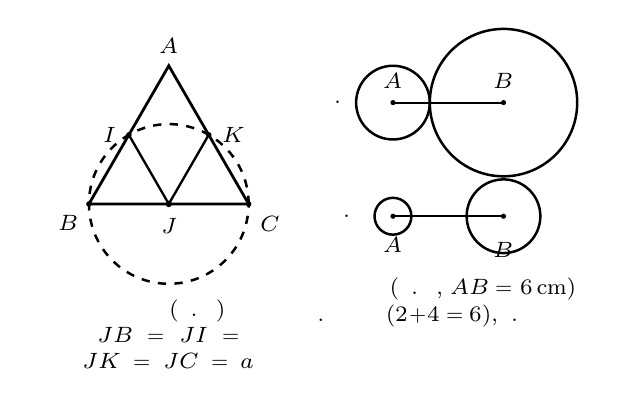
\begin{tikzpicture}[scale=0.78, every node/.style={font=\footnotesize, text=black}]
  % ឆ្វេង៖ លំហាត់ទី៦ ទំ.២០៤ (ត្រីកោណសម័ង្ស ABC => B,I,K,C នៅលើរង្វង់ផ្ចិត J)
  \begin{scope}[shift={(0,0)}]
    \coordinate (B) at (0.20,0.45);
    \coordinate (C) at (2.80,0.45);
    \coordinate (A) at (1.50,2.70);
    \coordinate (J) at (1.50,0.45);
    \coordinate (I) at ($(A)!0.5!(B)$);
    \coordinate (K) at ($(A)!0.5!(C)$);
    \draw[black, line width=0.90pt, dashed] (J) circle (1.30);
    \draw[black, line width=1.0pt] (A)--(B)--(C)--cycle;
    \draw[black, line width=0.85pt] (J)--(I) (J)--(K);
    \fill[black] (J) circle (1.5pt) node[below=1.5pt] {$J$};
    \fill[black] (B) circle (1.3pt) node[below left=1pt] {$B$};
    \fill[black] (C) circle (1.3pt) node[below right=1pt] {$C$};
    \fill[black] (I) circle (1.3pt) node[left=1.5pt] {$I$};
    \fill[black] (K) circle (1.3pt) node[right=1.5pt] {$K$};
    \node[above=1pt] at (A) {$A$};
    \node[anchor=north, text width=3.35cm, align=center] at (1.50,-0.95) {លំហាត់ទី៦ (ទំ.២០៤)៖\\$JB=JI=JK=JC=a$};
  \end{scope}
  % ស្ដាំ៖ ប្រតិបត្តិ ក, ខ, គ (ទំ.១៩៨) AB = 6 cm
  \begin{scope}[shift={(4.45,0.20)}]
    % ក៖ ប៉ះក្រៅ (2+4=6)
    \coordinate (A1) at (0.70,1.90); \coordinate (B1) at (2.50,1.90);
    \draw[black, line width=0.9pt] (A1) circle (0.60);
    \draw[black, line width=0.9pt] (B1) circle (1.20);
    \draw[black, line width=0.8pt] (A1)--(B1);
    \fill[black] (A1) circle (1.2pt) node[above=1.5pt] {$A$};
    \fill[black] (B1) circle (1.2pt) node[above=1.5pt] {$B$};
    \node[left=2pt] at (0.10,1.90) {ក.};
    % គ៖ ដាច់ពីគ្នា (1+2 < 6)
    \coordinate (A2) at (0.70,0.05); \coordinate (B2) at (2.50,0.05);
    \draw[black, line width=0.9pt] (A2) circle (0.30);
    \draw[black, line width=0.9pt] (B2) circle (0.60);
    \draw[black, line width=0.8pt] (A2)--(B2);
    \fill[black] (A2) circle (1.2pt) node[below=4pt] {$A$};
    \fill[black] (B2) circle (1.2pt) node[below=6pt] {$B$};
    \node[left=2pt] at (0.25,0.05) {គ.};
    \node[anchor=north, text width=3.55cm, align=center] at (1.65,-0.80) {ប្រតិបត្តិ (ទំ.១៩៨, $AB=6\unit{cm}$)៖\\ក. ប៉ះក្រៅ ($2+4=6$), គ. ដាច់ពីគ្នា};
  \end{scope}
\end{tikzpicture}}

\begin{document}
\fontsize{10pt}{15.2pt}\selectfont

% -------------------- ក្បាលកិច្ចតែងការ (Header) --------------------
\begin{center}
  {\muol\fontsize{11pt}{16pt}\selectfont ព្រះរាជាណាចក្រកម្ពុជា}\\[2pt]
  {\muol\fontsize{10pt}{15pt}\selectfont ជាតិ សាសនា ព្រះមហាក្សត្រ}\\[1pt]
  \khmflourish
\end{center}

\vspace{-28pt}
{\muol\fontsize{9.5pt}{12.5pt}\selectfont
មន្ទីរអប់រំ យុវជន និងកីឡា ខេត្តកំពង់ធំ\\
ការិយាល័យអប់រំ យុវជន និងកីឡា ស្រុកកំពង់ស្វាយ\\
អនុវិទ្យាល័យព្រះក្រសាំង}

\vspace{1pt}
\begin{center}
  {\muol\fontsize{10pt}{14pt}\selectfont កិច្ចតែងការបង្រៀន}
\end{center}
\vspace{0pt}

% -------------------- ព័ត៌មានទូទៅ (Metadata) --------------------
{\renewcommand{\arraystretch}{0.95}
\hspace*{4.05cm}%
\begin{tabular}{@{}l l l@{}}
  - \hspace{0.35cm} មុខវិជ្ជា & : & គណិតវិទ្យា ថ្នាក់ទី៨ \\
  - \hspace{0.35cm} ចំណងជើងមេរៀន & : & មេរៀនទី១៥ រង្វង់ \\
  - \hspace{0.35cm} ចំណងជើងរង & : & ១. សញ្ញាណរង្វង់ និងការកំណត់រង្វង់ (ទំ.១៩៧--១៩៨ និងទំ.២០៤) \\
  - \hspace{0.35cm} រយៈពេល & : & ១ ម៉ោងសិក្សា (៥០ នាទី) \\
  - \hspace{0.35cm} បង្រៀនដោយ & : & ហុក ប៊ុនថែន \\
  - \hspace{0.35cm} កាលបរិច្ឆេទ & : & ថ្ងៃព្រហស្បតិ៍ ១៥កើត ខែមិគសិរ ព.ស.២៥៧០ (២៤ ធ្នូ ២០២៦) \\
\end{tabular}
}

\vspace{1pt}

% -------------------- I. វត្ថុបំណង --------------------
\textbf{I.} {\muol វត្ថុបំណង}\\[1pt]
\hspace*{0.55cm}%
\begin{tabular}{@{}l l L{14.2cm}@{}}
  \wcirc \hspace{0.25cm} វិជ្ជាសម្បទា & : & សិស្សពោលបានត្រឹមត្រូវនូវនិយមន័យរង្វង់ $C(O,r)$ ធាតុសំខាន់ៗនៃរង្វង់ (ផ្ចិត $O$ កាំ $r$ អង្កត់ធ្នូ និងអង្កត់ផ្ចិត $d=2r$) ព្រមទាំងទ្រឹស្ដីបទនៃការកំណត់រង្វង់តែមួយគត់កាត់តាមបីចំណុចមិនស្ថិតនៅលើបន្ទាត់តែមួយ តាមសៀវភៅគោល ទំ.១៩៧--១៩៨ ។ \\
  \wcirc \hspace{0.25cm} បំណិនសម្បទា & : & សិស្សសង់រកផ្ចិតរង្វង់ $O$ តាមប្រសព្វមេដ្យាទ័រពីរលើសន្លឹកកិច្ចការស-ខ្មៅ ស្រាយបញ្ជាក់ថាចំណុច ៣ ឬ ៤ ស្ថិតនៅលើរង្វង់តែមួយតាមលក្ខខណ្ឌចម្ងាយស្មើគ្នាពីផ្ចិត និងកំណត់ទីតាំងធៀបនៃរង្វង់ពីរ ($C(A,r_1)$ និង $C(B,r_2)$) បានត្រឹមត្រូវ ។ \\
  \wcirc \hspace{0.25cm} ចរិយាសម្បទា & : & សិស្សមានទម្លាប់ផ្ទៀងផ្ទាត់លក្ខខណ្ឌចម្ងាយស្មើគ្នាដោយដែកឈាន និងបន្ទាត់ក្រិត មិនស្មានយកចំណុចកណ្ដាលអង្កត់ធ្នូជាផ្ចិតរង្វង់ដោយគ្មានអង្កត់ផ្ចិត និងឃើញតម្លៃអនុវត្តក្នុងបុរាណវិទ្យា និងសិប្បកម្ម ។ \\
\end{tabular}

\vspace{1pt}

% -------------------- II. សម្ភារៈឧបទេស --------------------
\textbf{II.} {\muol សម្ភារៈឧបទេស}\\[1pt]
\hspace*{0.55cm}$\bullet$ \hspace{0.35cm} សៀវភៅសិក្សាគោលគណិតវិទ្យាថ្នាក់ទី៨ (ទំ.១៩៧--១៩៨ និងទំ.២០៤) ក្ដារខៀន ដីស បន្ទាត់ក្រិត ដែកឈាន និងសន្លឹកកិច្ចការសិស្សស-ខ្មៅ (\en{Worksheet\_CIRC1} ចំនួន ២ ទំព័រ \en{A4} ដោយគ្មានស្លាយ \en{LCD}) ។

\vspace{1pt}

% -------------------- III. វិធីសាស្រ្តបង្រៀន --------------------
\textbf{III.} {\muol វិធីសាស្រ្តបង្រៀន}\\[1pt]
\hspace*{0.55cm}$\bullet$ \hspace{0.35cm} គោលវិធីសិស្សមជ្ឈមណ្ឌលតាមគំរូ \en{5Es} រួមបញ្ចូល \textbf{វិធីរុករកសំណុំចំណុចស្មើចម្ងាយតាមការបន្ថែមលក្ខខណ្ឌ ១$\to$២$\to$៣ ចំណុច} (\en{Progressive Locus-of-Equidistance Inquiry}, \en{Gutiérrez et al., 2021}) និងការបំពេញសន្លឹកកិច្ចការជាដៃគូ ។

\vspace{2pt}

% -------------------- IV. ដំណើរការបង្រៀន --------------------
\textbf{IV.} {\muol ដំណើរការបង្រៀន}\\[-6pt]

{\renewcommand{\arraystretch}{1.15}
\begin{longtable}{|L{5.50cm}|L{7.90cm}|L{4.80cm}|}
\hline
\multicolumn{1}{|c|}{\cellcolor{headgray}\muol សកម្មភាពគ្រូ} &
\multicolumn{1}{c|}{\cellcolor{headgray}\muol ខ្លឹមសារមេរៀន} &
\multicolumn{1}{c|}{\cellcolor{headgray}\muol សកម្មភាពសិស្ស} \\[2pt]
\hline
\endfirsthead

\hline
\multicolumn{1}{|c|}{\cellcolor{headgray}\muol សកម្មភាពគ្រូ} &
\multicolumn{1}{c|}{\cellcolor{headgray}\muol ខ្លឹមសារមេរៀន} &
\multicolumn{1}{c|}{\cellcolor{headgray}\muol សកម្មភាពសិស្ស} \\[2pt]
\hline
\endhead

\hline
\endfoot

% ==================== ជំហានទី១ (2min) ====================
\stepheader{ជំហានទី១ ៖ រដ្ឋបាលថ្នាក់ (២ នាទី)}
$\bullet$ ពិនិត្យអវត្តមាន សណ្ដាប់ធ្នាប់ អនាម័យ និងការត្រៀមដែកឈាន-បន្ទាត់ក្រិត \par\vspace{1pt}
$\bullet$ ចែកសន្លឹកកិច្ចការស-ខ្មៅ \en{Worksheet\_CIRC1} (១ សន្លឹកសងខាងក្នុងម្នាក់)
&
$\bullet$ វត្តមានសិស្ស វិន័យ និងការត្រៀមសម្ភារៈធរណីមាត្រ \par\vspace{1pt}
$\bullet$ សន្លឹកកិច្ចការសិស្ស \en{Worksheet\_CIRC1} (មេរៀនទី១៥ ៖ ១. រង្វង់)
&
$\circ$ ប្រធានថ្នាក់រាយការណ៍អវត្តមាន \par\vspace{1pt}
$\circ$ ទទួលសន្លឹកកិច្ចការ សរសេរឈ្មោះ និងដាក់ដែកឈានលើតុ \\
\hline

% ==================== ជំហានទី២ (9min) ====================
\stepheader{ជំហានទី២ ៖ កែកិច្ចការផ្ទះ រំលឹកមេរៀនចាស់ និងភ្ជាប់បញ្ហាថ្មី (៩ នាទី)}
\timenote{(កែកិច្ចការផ្ទះ $\le 3\unit{min}$)} \par
$\bullet$ ហៅសិស្ស ១ នាក់ឡើងបង្ហាញចម្លើយសង្ខេបនៃលំហាត់ទី៧ (មេរៀនទី១៤ ទំ.១៩៦) លើក្ដារខៀន
&
\textbf{កំណែកិច្ចការផ្ទះ (មេរៀនទី១៤ ទំ.១៩៦ — លំហាត់ទី៧)៖} \par
$\bullet$ ចតុកោណព្នាយ ($b'=15, b=30, h=15$)៖ \par
\hspace*{0.3em}$S = \dfrac{(15+30)\times 15}{2} = \dfrac{45\times 15}{2} = \mathbf{337.5}$ (ឯកតាផ្ទៃ) ។
&
$\circ$ ផ្ទៀងផ្ទាត់ចម្លើយក្នុងសៀវភៅលំហាត់ និងកែលម្អកំហុសឆ្គង \\[3pt]

\timenote{(រំលឹកមេរៀនទាក់ទង $3\unit{min}$)} \par
$\bullet$ សួររំលឹកលក្ខណៈ \textbf{មេដ្យាទ័រនៃអង្កត់} (មេរៀនទី១២) និង \textbf{មេដ្យានត្រីកោណកែង} (មេរៀនទី១៣)
&
\textbf{រំលឹកចំណេះដឹងមូលដ្ឋានភ្ជាប់មេរៀនទី១៥៖} \par
១. បន្ទាត់ $d$ ជាមេដ្យាទ័រនៃអង្កត់ $AB \iff d \perp AB$ ត្រង់ចំណុចកណ្ដាល $I$ ហើយគ្រប់ចំណុច $M \in d \iff \mathbf{MA = MB}$ ។ \par
២. ក្នុងត្រីកោណកែង $\tri{ABC}$ ($\ang{B}=90^\circ$) មេដ្យាន $BO = \frac{1}{2}AC \Rightarrow OA = OB = OC$ ។
&
$\circ$ ឆ្លើយរំលឹក៖ «គ្រប់ចំណុចលើមេដ្យាទ័រនៃ $AB$ មានចម្ងាយស្មើទៅចុងទាំងពីរ $A$ និង $B$» \\[3pt]

\fiveE{E1 - Engage} \timenote{(3 min)} \par
$\bullet$ លើកបេសកកម្ម \textbf{«បំណែកគែមចានបុរាណបាក់»} លើក្ដារខៀន និងផ្នែកទី១ នៃសន្លឹកកិច្ចការ \par
\hspace*{0.3em}– សំណួរ៖ «បើយកចំណុចកណ្ដាលនៃ $AC$ ធ្វើជាផ្ចិត $O$ តើចម្ងាយទៅ $B$ ស្មើគ្នាជានិច្ចឬទេ?»
&
\textbf{បេសកកម្ម E1 ៖ បំណែកគែមចានបុរាណនៅកំពង់ធំ} \par
អ្នកបុរាណវិទ្យារកឃើញបំណែកគែមចានរាងរង្វង់ដែលបាត់ផ្នែកកណ្ដាល ដោយដៅចំណុចគែម $A, B, C$ ។ \par
$\bullet$ \textbf{មតិទី១៖} យកចំណុចកណ្ដាលនៃ $AC$ ធ្វើជាផ្ចិត $O$ ។ \par
$\bullet$ \textbf{មតិទី២៖} សង់ប្រសព្វមេដ្យាទ័រនៃ $AB$ និង $BC$ ។ \par
(ទុកផ្ទៀងផ្ទាត់ដោយដែកឈាននៅ \en{E2} និងបិទបញ្ចប់នៅ \en{E5})
&
$\circ$ អានបេសកកម្មលើសន្លឹកកិច្ចការ និងគូសធីកទស្សន៍ទាយមតិទី១ ឬមតិទី២ \\[3pt]

&
\cfig{\figEngageCIRCOne}
& \\[3pt]
\hline

% ==================== ជំហានទី៣ (17min) ====================
\stepheader{ជំហានទី៣ ៖ មេរៀនថ្មី — សញ្ញាណរង្វង់ និងការកំណត់រង្វង់ (១៧ នាទី)}
\fiveE{E2 - Explore} \timenote{(11 min)} \par
\ditem \textbf{សកម្មភាពទី១៖ ធាតុនៃរង្វង់ និងការគូសកាត់ ១--២ ចំណុច ($5\unit{min}$)} \par
$\bullet$ ឱ្យសិស្សពិនិត្យរូបទី១ (ខ្នាតពិត $1:1$, កាំ $r=1.5\unit{cm}$) ក្នុងផ្នែកទី២ នៃសន្លឹកកិច្ចការ វាស់ $OA, OB, OC$ និងសម្គាល់ឈ្មោះអង្កត់ $AB$ និង $AC$
&
\textbf{១. រុករកធាតុនៃរង្វង់ និងចំនួនរង្វង់កាត់តាម ១ ឬ ២ ចំណុច៖} \par
$\bullet$ វាស់លើរូបខ្នាតពិត $1:1$៖ $OA = OB = OC = 1.5\unit{cm}$ (កាំ $r$) និងអង្កត់ផ្ចិត $AC = 3.0\unit{cm} = 2r$ ។ \par
$\bullet$ \textbf{ឧទាហរណ៍ទី១ (ទំ.១៩៧ — កាត់តាម ១ ចំណុច $A$)៖} គូសបានរង្វង់ \textbf{ច្រើនរាប់មិនអស់} (ផ្ចិត $O_1, O_2, O_3\dots$ ស្ថិតនៅគ្រប់ទីកន្លែងក្នុងប្លង់) ។ \par
$\bullet$ \textbf{ឧទាហរណ៍ទី២ (ទំ.១៩៨ — កាត់តាម ២ ចំណុច $A, B$)៖} ដើម្បីឱ្យ $OA = OB$ ផ្ចិតទាំងអស់ត្រូវស្ថិតលើ \textbf{មេដ្យាទ័រនៃអង្កត់ $AB$} $\Rightarrow$ គូសបានរង្វង់ \textbf{ច្រើនរាប់មិនអស់} ។
&
$\circ$ ប្រើបន្ទាត់ក្រិតវាស់ឃើញ $OA=OB=OC=1.5\unit{cm}$ និង $AC=3.0\unit{cm}$ \par\vspace{1pt}
$\circ$ សាកល្បងចាក់ដែកឈានគូសរង្វង់កាត់តាម $A, B$ ដោយដាក់ផ្ចិតលើមេដ្យាទ័រនៃ $AB$ \\[3pt]

\ditem \textbf{សកម្មភាពទី២៖ កាត់តាម ៣ ចំណុច និងអន្ទាក់ការយល់ច្រឡំ ($6\unit{min}$)} \par
$\bullet$ ឱ្យដៃគូសិស្សពិនិត្យរូបបំណែកចាន $A, B, C$ ខ្នាតពិត $1:1$៖ \par
\hspace*{0.3em}– សាកវាស់ចម្ងាយពីចំណុចកណ្ដាល $I$ នៃ $AC$ ទៅ $A, C, B$ (អន្ទាក់ទី១) \par
\hspace*{0.3em}– ប្រើប្រសព្វមេដ្យាទ័រ $O = d_1 \cap d_2$ រួចចាក់ដែកឈានគូសរង្វង់ និងពិនិត្យករណី $A, B, C$ រត់ត្រង់គ្នា (អន្ទាក់ទី២)
&
\textbf{២. រុករកករណី ៣ ចំណុច និងអន្ទាក់ការយល់ច្រឡំទាំង ២៖} \par
$\bullet$ \textbf{អន្ទាក់ទី១ (ចំណុចកណ្ដាល $I$ នៃ $AC$)៖} វាស់ឃើញ $IA = IC$ ប៉ុន្តែ $IB \ne IA$ (ព្រោះ $AC$ គ្រាន់តែជាអង្កត់ធ្នូ មិនមែនអង្កត់ផ្ចិតទេ!) ។ \par
$\bullet$ \textbf{ឧទាហរណ៍ទី៣ (ទំ.១៩៨ — ៣ ចំណុចមិនរត់ត្រង់គ្នា)៖} មេដ្យាទ័រ $d_1$ នៃ $AB$ និងមេដ្យាទ័រ $d_2$ នៃ $BC$ ប្រសព្វគ្នាត្រង់ \textbf{ចំណុច $O$ តែមួយគត់} ដែល $OA = OB = OC \Rightarrow$ គូសបាន \textbf{រង្វង់តែមួយគត់} ។ \par
$\bullet$ \textbf{អន្ទាក់ទី២ ($A, B, C$ រត់ត្រង់គ្នា)៖} មេដ្យាទ័រនៃ $AB$ និង $BC$ កែងនឹងបន្ទាត់តែមួយ $\Rightarrow d_1 \parallel d_2$ (គ្មានចំណុចប្រសព្វ) $\Rightarrow$ \textbf{មិនអាចគូសរង្វង់បានទេ} ។
&
$\circ$ វាស់ឃើញ $IB \ne IA$ បដិសេធមតិទី១ \par\vspace{1pt}
$\circ$ ចាក់ដែកឈានត្រង់ $O = d_1\cap d_2$ គូសរង្វង់កាត់តាម $A, B, C$ គត់ល្អ និងពន្យល់ហេតុផល $d_1\parallel d_2$ ពេលរត់ត្រង់គ្នា \\[3pt]

&
\cfig{\figExploreLocusCIRCOne}
& \\[3pt]

\fiveE{E3 - Explain} \timenote{(6 min)} \par
$\bullet$ សំយោគនិយមន័យ ទ្រឹស្ដីបទ និងចំណាំតាមសៀវភៅគោល ទំ.១៩៧--១៩៨ លើក្ដារខៀន
&
{\muol ១. រង្វង់ — ១.១ និយមន័យ និង ១.២ ការកំណត់រង្វង់ (ទំ.១៩៧--១៩៨)} \par
$\bullet$ \textbf{និយមន័យ៖} សំណុំចំណុចក្នុងប្លង់ដែលមានចម្ងាយស្មើនឹង $r$ ($r>0$) ពីចំណុចថេរ $O$ ហៅថា \textbf{រង្វង់} ផ្ចិត $O$ កាំ $r$ កំណត់សរសេរ $C(O, r)$ ។ \par
\hspace*{0.3em}– \textbf{កាំ ($r$)៖} អង្កត់ភ្ជាប់ផ្ចិត $O$ ទៅចំណុចលើរង្វង់ ($OA = r$) ។ \par
\hspace*{0.3em}– \textbf{អង្កត់ធ្នូ៖} អង្កត់ភ្ជាប់ពីរចំណុចលើរង្វង់ ($AB$) ។ \textbf{អង្កត់ផ្ចិត៖} អង្កត់ធ្នូកាត់តាមផ្ចិត $O$ ($AC = 2r$) ។
&
$\circ$ បំពេញនិយមន័យរង្វង់ កាំ អង្កត់ធ្នូ និងអង្កត់ផ្ចិតក្នុងផ្នែកទី៣ នៃសន្លឹកកិច្ចការ \\[3pt]

$\bullet$ សរសេរទ្រឹស្ដីបទ និងសម្គាល់ការកំណត់រង្វង់លើក្ដារខៀន
&
$\bullet$ \textbf{ទ្រឹស្ដីបទ (ទំ.១៩៨)៖} តាមបីចំណុចដែលមិនស្ថិតនៅលើបន្ទាត់តែមួយ គេអាចគូសបាន \textbf{រង្វង់តែមួយគត់} ដែលកាត់តាមចំណុចទាំងនោះ (ផ្ចិត $O$ ជាប្រសព្វមេដ្យាទ័រនៃជ្រុងត្រីកោណ $ABC$) ។ \par
$\bullet$ \textbf{សម្គាល់៖} បើបីចំណុចស្ថិតនៅលើបន្ទាត់តែមួយ គេមិនអាចគូសរង្វង់កាត់តាមចំណុចទាំងបីនោះបានទេ ។
&
$\circ$ កត់ត្រាទ្រឹស្ដីបទ និងចំណាំចូលក្នុងសន្លឹកកិច្ចការ \\[3pt]

&
\cfig{\figCircleDefDet}
& \\[3pt]

$\bullet$ ណែនាំធនាគារហេតុផល \cnum{1}--\cnum{5} លើក្ដារខៀនសម្រាប់ការស្រាយបញ្ជាក់
&
{\fontsize{9.2pt}{13pt}\selectfont
\begin{tabular}[t]{|L{7.55cm}|}
\hline
\cellcolor{headgray}\textbf{ធនាគារហេតុផល (\en{Warrant Bank}) សម្រាប់សញ្ញាណ និងការកំណត់រង្វង់} \\[2pt]
\hline
\cnum{1} និយមន័យរង្វង់ $C(O,r)$៖ $M \in C(O,r) \iff OM = r$ (ចំណុចច្រើននៅលើរង្វង់តែមួយ $\iff$ ស្មើចម្ងាយពីផ្ចិត $O$ តែមួយ) \par
\cnum{2} ទំនាក់ទំនងអង្កត់ផ្ចិត និងកាំ៖ $d = 2r \iff r = \dfrac{d}{2}$ \par
\cnum{3} លក្ខណៈមេដ្យាទ័រនៃអង្កត់៖ $O \in \text{មេដ្យាទ័រនៃ } AB \iff OA = OB$ \par
\cnum{4} ទ្រឹស្ដីបទរង្វង់កាត់តាម ៣ ចំណុចមិនរត់ត្រង់គ្នា ($O = MN \cap PQ$) \par
\cnum{5} ទីតាំងរង្វង់ពីរ $C(A,r_1)$ និង $C(B,r_2)$៖ ប៉ះក្រៅ ($AB=r_1+r_2$), ប្រសព្វគ្នា ($|r_1-r_2|<AB<r_1+r_2$), ដាច់ពីគ្នា ($AB>r_1+r_2$) \\[2pt]
\hline
\end{tabular}}\par\vspace{2pt}
&
$\circ$ ផ្ទៀងផ្ទាត់លេខកូដហេតុផល \cnum{1}--\cnum{5} លើសន្លឹកកិច្ចការ \\
\hline

% ==================== ជំហានទី៤ (20min) ====================
\stepheader{ជំហានទី៤ ៖ ពង្រឹងចំណេះដឹង និងវាយតម្លៃ (២០ នាទី)}
\fiveE{E4 - Elaborate} \timenote{(10 min)} \par
\ditem \textbf{គំរូទី១៖ លំហាត់គំរូសៀវភៅគោល ទំ.១៩៨ ($5\unit{min}$)} \par
$\bullet$ ដឹកនាំសិស្សបំពេញសម្រាយបញ្ជាក់ថា ៣ ចំណុច $A, B, C$ មិនរត់ត្រង់គ្នាស្ថិតនៅលើរង្វង់តែមួយ ក្នុងផ្នែកទី៤ នៃសន្លឹកកិច្ចការ
&
\textbf{លំហាត់គំរូទី១ (ទំ.១៩៨ — សម្រាយបញ្ជាក់ទ្រឹស្ដីបទ)៖} \par
គេមានបីចំណុច $A, B, C$ មិនស្ថិតលើបន្ទាត់តែមួយ ។ ស្រាយថា $A, B, C$ ស្ថិតលើរង្វង់តែមួយគត់ ។ \par
$\bullet$ យក $MN$ ជាមេដ្យាទ័រនៃ $AC$ និង $PQ$ ជាមេដ្យាទ័រនៃ $AB$ ។ \par
$\bullet$ ដោយ $A, B, C$ មិនរត់ត្រង់គ្នា នោះ $MN$ និង $PQ$ ប្រសព្វគ្នាត្រង់ចំណុច $O$ តែមួយគត់៖ \par
\hspace*{0.3em}– $O \in MN \Rightarrow OA = OC$ (តាម \cnum{3}) ។ \par
\hspace*{0.3em}– $O \in PQ \Rightarrow OA = OB$ (តាម \cnum{3}) ។ \par
$\bullet$ ដូចនេះ $OA = OB = OC = r \Rightarrow$ រង្វង់ $C(O, OA)$ ជា \textbf{រង្វង់តែមួយគត់} កាត់តាម $A, B, C$ (តាម \cnum{1}, \cnum{4}) ។
&
$\circ$ បំពេញចន្លោះសម្រាយបញ្ជាក់ និងដាក់លេខហេតុផល \cnum{3}, \cnum{1} លើសន្លឹកកិច្ចការ \\[3pt]

\ditem \textbf{គំរូទី២៖ ស្រាយបញ្ជាក់ ៤ ចំណុចលើរង្វង់តែមួយ — លំហាត់ទី៦ ទំ.២០៤ ($5\unit{min}$)} \par
$\bullet$ ណែនាំយុទ្ធវិធីភ្ជាប់បាតមធ្យមត្រីកោណ (មេរៀនទី១៣) ដើម្បីបង្ហាញថា $B, I, K, C$ មានចម្ងាយស្មើពី $J$
&
\textbf{គំរូទី២ (លំហាត់ទី៦ ទំ.២០៤ — ៤ ចំណុចលើរង្វង់តែមួយ)៖} \par
ត្រីកោណសម័ង្ស $\tri{ABC}$ (ជ្រុងស្មើ $2a$) មាន $I, J, K$ ជាចំណុចកណ្ដាលនៃ $AB, BC, CA$ ។ ស្រាយថា $B, I, K, C$ ស្ថិតលើរង្វង់ផ្ចិត $J$ ។ \par
$\bullet$ $J$ ជាចំណុចកណ្ដាល $BC \Rightarrow JB = JC = \frac{1}{2}BC = a$ ។ \par
$\bullet$ $IJ$ និង $JK$ ជាបាតមធ្យមនៃ $\tri{ABC}$៖ \par
\hspace*{0.3em}$JI = \frac{1}{2}AC = a$ និង $JK = \frac{1}{2}AB = a$ ។ \par
$\bullet$ ដូចនេះ $JB = JI = JK = JC = a \Rightarrow$ ចំណុចទាំងបួន $B, I, K, C$ ស្ថិតនៅលើរង្វង់តែមួយ $C(J, a)$ (តាម \cnum{1}) ។
&
$\circ$ ប្រើបាតមធ្យមត្រីកោណគណនាឃើញ $JB=JI=JK=JC=a$ រួចសន្និដ្ឋានតាម \cnum{1} \\[3pt]

&
\cfig{\figPractCIRCOne}
& \\[3pt]

\fiveE{E5 - Evaluate} \timenote{(10 min)} \par
\ditem \textbf{ប្រតិបត្តិសៀវភៅគោល ទំ.១៩៨ ក, ខ, គ ($6.5\unit{min}$)៖} \par
$\bullet$ ឱ្យសិស្សបំពេញតារាងប្រៀបធៀប $AB = 6\unit{cm}$ ទៅនឹង $r_1 + r_2$ និងគូសរង្វង់លើអ័ក្សខ្នាតក្រិតក្នុងផ្នែកទី៥ នៃសន្លឹកកិច្ចការ រួចផ្ទៀងជាដៃគូ
&
\textbf{ប្រតិបត្តិ (ទំ.១៩៨ — អង្កត់ $AB = 6\unit{cm}$)៖} \par
$\bullet$ \textbf{ក. $C(A, 2\unit{cm})$ និង $C(B, 4\unit{cm})$៖} $r_1 + r_2 = 2 + 4 = 6\unit{cm} = AB \Rightarrow$ រង្វង់ទាំងពីរ \textbf{ប៉ះគ្នាខាងក្រៅ} (មាន ១ ចំណុចរួមលើ $AB$) ។ \par
$\bullet$ \textbf{ខ. $C(A, 3\unit{cm})$ និង $C(B, 5\unit{cm})$៖} $5-3 < 6 < 3+5$ ($2 < 6 < 8$) $\Rightarrow$ រង្វង់ទាំងពីរ \textbf{ប្រសព្វគ្នាត្រង់ ២ ចំណុច} ។ \par
$\bullet$ \textbf{គ. $C(A, 1\unit{cm})$ និង $C(B, 2\unit{cm})$៖} $r_1 + r_2 = 1 + 2 = 3\unit{cm} < 6\unit{cm} \Rightarrow$ រង្វង់ទាំងពីរ \textbf{ដាច់ពីគ្នាខាងក្រៅ} (គ្មានចំណុចរួម) ។
&
$\circ$ គណនាផលបូកកាំ $r_1+r_2$ គូសរង្វង់ដោយដែកឈាន និងផ្ទៀងចម្លើយជាមួយដៃគូ \\[3pt]

\ditem \textbf{បិទបេសកកម្ម E1 និងតេស្តរហ័ស \en{Exit Check} ($3.5\unit{min}$)៖} \par
$\bullet$ សួរបិទបេសកកម្មបំណែកចានបុរាណ និងឱ្យសិស្សជ្រើសរើស \en{A--D}
&
$\bullet$ \textbf{បិទបេសកកម្ម E1៖} ត្រូវប្រើ \textbf{មតិទី២} (ប្រសព្វមេដ្យាទ័រនៃ $AB$ និង $BC$) ទើបរកឃើញផ្ចិតដើម $O$ តែមួយគត់នៃចានបុរាណ ។ \par
$\bullet$ \textbf{Exit Check៖} តើគេអាចគូសរង្វង់បានប៉ុន្មានកាត់តាម ៣ ចំណុច $M, N, P$ ដែលរត់ត្រង់គ្នាលើបន្ទាត់តែមួយ? \par
\graybox{\enbf{A.} មិនអាចគូសបាន ($0$ រង្វង់) \ding{51}} \quad \en{B.} $1$ រង្វង់ \quad \en{C.} $2$ រង្វង់ \quad \en{D.} រាប់មិនអស់
&
$\circ$ លើកម្រាមដៃទី១ ជ្រើសរើស \textbf{A ($0$ រង្វង់)} ព្រោះមេដ្យាទ័រទាំងពីរស្របគ្នា \\
\hline

% ==================== ជំហានទី៥ (<=2min) ====================
\stepheader{ជំហានទី៥ ៖ កិច្ចការផ្ទះ និងបណ្ដាំផ្ញើ ($\le$ ២ នាទី)}
$\bullet$ កត់ត្រាកិច្ចការផ្ទះលើក្ដារខៀន (មានបោះពុម្ពស្រាប់នៅផ្នែកទី៦ នៃសន្លឹកកិច្ចការទំព័រទី២)
&
\textbf{កិច្ចការផ្ទះ (សៀវភៅសិក្សាគោល ទំ.១៩៨ និងទំ.២០៤)៖} \par
១. \textbf{លំហាត់ទី៧ (ទំ.២០៤)៖} ចតុកោណ $ABCD$ មានអង្កត់ទ្រូងកែងគ្នា ($AC \perp BD$) ។ $M, N, R, S$ ជាចំណុចកណ្ដាលរៀងគ្នានៃ $AB, BC, CD, DA$ ។ ស្រាយបំភ្លឺថាចំណុចទាំងបួន $M, N, R, S$ ស្ថិតនៅលើរង្វង់តែមួយ (\textit{ណែនាំ៖ បង្ហាញថា $MNRS$ ជាចតុកោណកែងមានប្រសព្វអង្កត់ទ្រូង $O$}) ។ \par
២. សង់រូប \textbf{ប្រតិបត្តិ ក, ខ, គ (ទំ.១៩៨)} តាមខ្នាតពិត $AB = 6\unit{cm}$ ក្នុងសៀវភៅលំហាត់ ។
&
$\circ$ កត់ត្រាកិច្ចការផ្ទះ និងទុកដាក់សន្លឹកកិច្ចការក្នុងសៀវភៅសរសេរ \\[3pt]

$\bullet$ ណែនាំឱ្យអានចំណុចបន្ទាប់ជាមុន និងផ្ដាំផ្ញើត្រៀមឧបករណ៍ធរណីមាត្រ
&
$\bullet$ \textbf{អានជាមុន៖} ចំណុច \textbf{២. មុំ និងធ្នូ — ២.១ មុំផ្ចិត} (ទំព័រ ១៩៩--២០០) ។ \par
$\bullet$ \textbf{បណ្ដាំផ្ញើ៖} ត្រៀមបន្ទាត់ក្រិត ដែកឈាន និងរ៉ាប់ព័រទ័រសម្រាប់វាស់មុំផ្ចិតនៅម៉ោងក្រោយ ។
&
$\circ$ ទទួលបណ្ដាំផ្ញើ និងជម្រាបលាគ្រូ \\

\end{longtable}
}

\vspace{8pt}

% -------------------- ហត្ថលេខា (Signature Block) --------------------
\begin{flushright}
\begin{minipage}{9.6cm}
\centering
ថ្ងៃព្រហស្បតិ៍ ១៥កើត ខែមិគសិរ ឆ្នាំមមី អដ្ឋស័ក ពុទ្ធសករាជ ២៥៧០\\[2pt]
ព្រះក្រសាំង, ថ្ងៃទី២៤ ខែធ្នូ ឆ្នាំ២០២៦\\[4pt]
{\muol គ្រូបង្រៀន}\\[32pt]
\hfill{\muol ហុក ប៊ុនថែន}\hspace*{1.4cm}
\end{minipage}
\end{flushright}

\end{document}
